\documentclass[12pt,landscape]{article}
\usepackage{csvsimple}
\usepackage{graphicx}
\usepackage{hyperref}
\parindent=0pt
\setlength{\textwidth=9.5in}
\setlength{\oddsidemargin=-.25 in}
\setlength{\topmargin=0 in}
\setlength{\textheight=6 in}
\title{DUNE Offline Computing Model Calculations}
\author{H. Schellman for the Computing Consortium}
\date{\today}
\begin{document}


\makeatletter
\csvset{
  autotabularright/.style={
    file=#1,
    after head=\csv@pretable\begin{tabular}{|*{\csv@columncount}{r|}}\csv@tablehead,
    table head=\hline\csvlinetotablerow\\\hline,
    late after line=\\,
    table foot=\\\hline,
    late after last line=\csv@tablefoot\end{tabular}\csv@posttable,
    command=\csvlinetotablerow},
}
\makeatother
\newcommand{\csvautotabularright}[2][]{\csvloop{autotabularright={#2},#1}}

\maketitle
\section{Introduction}

This is an annual projection for DUNE CPU and storage needs intended for use at the Computing Contribitions Board meeting in November 2022. It projects needs for 2023 onwards. 

The projection is done using codes at: \href{https://github.com/DUNE/CCB-data/tree/master/Numbers-2023}{https://github.com/DUNE/CCB-data/tree/master/Numbers-2023} from parameters stored in a json file. We use CPU and storage sizes derived from protoDUNE and simulation experience and apply them to projected numbers of events from the various DUNE detectors. 

Changes since the last report include:

\begin{itemize}
\item a later start for ProtoDUNE 2 running at CERN
\item use of slot time instead of CPU time as our codes often require more memory than is available for a single batch slot. 
\item revisions to near term use based on the 2022 experience
\end{itemize}

\section{Model Assumptions}
{\tt Detectors:} Detectors included in the calculation = {\tt ['SP', 'SP2', 'DP', 'PDVD', 'HD', 'VD', 'ND']} \\
{\tt Cap:} Cap on Raw data/year in PB = {\tt 30} \\
{\tt Base-Memory:} MB of memory per slot assumed as the average = {\tt 3000} \\
{\tt MaxYear:} Plot until year = {\tt 2028} \\
{\tt MinYear:} Plot starting with year = {\tt 2020} \\
{\tt Reprocess:} Number of years of data reprocessed when doing a new pass = {\tt {'SP': 3, 'DP': 3, 'SP2': 4, 'PDVD': 4, 'ProtoDUNEs': 4, 'VD': 100, 'HD': 100, 'FDs': 100, 'ND': 100, 'MARS': 1}} \\
{\tt PatternFraction:} Fraction of time taken in pattern recognition = {\tt {'SP': 0.7, 'SP2': 0.7, 'DP': 0.7, 'PDVD': 0.7, 'ProtoDUNEs': 0.7, 'HD': 0.1, 'VD': 0.1, 'FDs': 0.1, 'ND': 0.9, 'MARS': 0}} \\
{\tt TapeLifetimes:} Number of years kept on tape = {\tt {'Raw': 100, 'Test': 0.5, 'Reco': 15, 'Sim': 15}} \\
{\tt DiskLifetimes:} Number of years kept on disk = {\tt {'Raw': 2, 'Test': 0.5, 'Reco': 2, 'Sim': 2}} \\
{\tt TapeCopies:} Number of copies kept on tape = {\tt {'Raw': 2, 'Test': 1, 'Reco': 1, 'Sim': 1}} \\
{\tt DiskCopies:} Number of copies kept on disk = {\tt {'Raw': 1, 'Test': 1, 'Reco': 2, 'Sim': 1}} \\
{\tt PerYear:} Number of reprocessing done per year = {\tt {'Raw': 1, 'Test': 1, 'Reco': 1, 'Sim': 1, 'Events': 1, 'Sim-Events': 1, 'Reco-CPU': 1, 'Sim-CPU': 1, 'Analysis': 1, 'Analysis-CPU': 1}} \\
{\tt Cores:} Description of cores, efficiency and speed relative to 2020 vintage = {\tt {'Efficiency': 0.7, '2020Units': 1}} \\
{\tt kHEPSPEC06PerCPU:} kHEPSPEC06 per core assumed = {\tt 0.011} \\
{\tt SplitsYear:} Year CERN no longer responsible for disk or tape = {\tt 2027} \\
{\tt filename:} Input configuration file = {\tt Parameters\_2022-11-07-2040.json} \\
\section{Disk and Tape needs by source and site}
\begin{table}[h]
 \centering\csvautotabularright{DUNERSEUSAGE-2022-11-14.csv}
 \label{Cumulative-Tape}
\caption{Rucio report on storage usage 2022-11-14 from the Scotgrid Dashboard \href{https://dune.monitoring.edi.scotgrid.ac.uk/app/dashboards}{https://dune.monitoring.edi.scotgrid.ac.uk/app/dashboards}.}
 \end{table}
\begin{table}[h]
\centering\csvautotabularright{Disk_by_location.csv}\label{Cumulative-Disk
}
\caption{Disk requests by location. The top 4 lines show the source, the bottom 4 show the locations requested and the total request.}
\end{table}
\begin{table}[h]
\centering\csvautotabularright{Tape_by_location.csv}\label{Cumulative-Tape
}
\caption{Tape requests by location. The top 4 lines show the source, the bottom 4 show the locations requested and the total request.}
\end{table}
\begin{figure}[ht]
\centering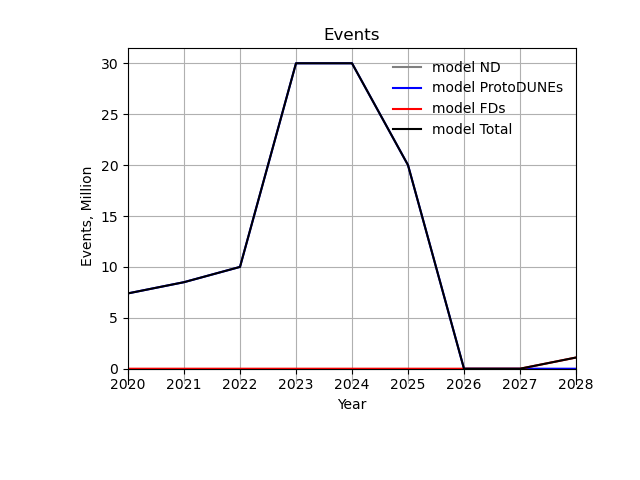
\includegraphics[height=0.4\textwidth]{report/Parameters_2022-11-07-2028-Events.png}\label{Events}
\caption{Million of detector events per year projected}
\end{figure}
\begin{figure}[ht]
\centering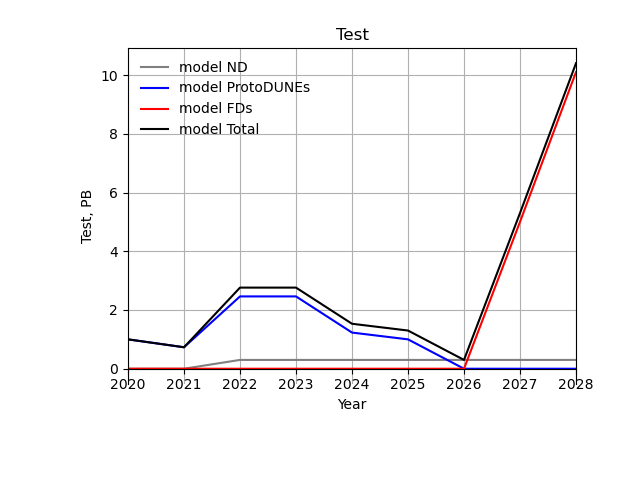
\includegraphics[height=0.4\textwidth]{report/Parameters_2022-11-07-2028-Test.png}\label{Test}
\caption{PB of Test data projected}
\end{figure}
\begin{figure}[ht]
\centering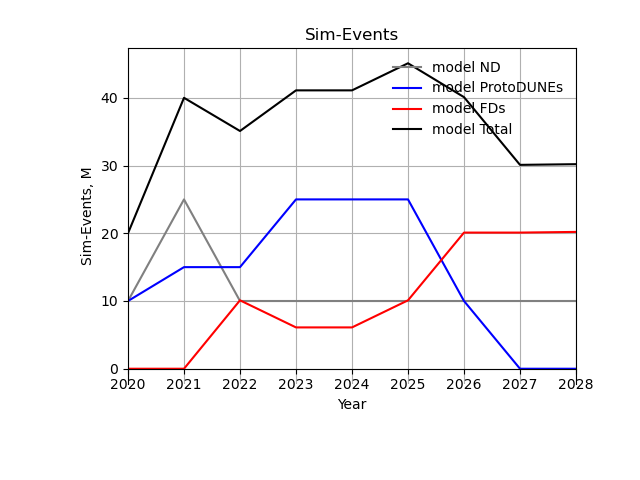
\includegraphics[height=0.4\textwidth]{report/Parameters_2022-11-07-2028-Sim-Events.png}\label{Sim-Events}
\caption{Millions of simulated events per year projected}
\end{figure}
\begin{figure}[ht]
\centering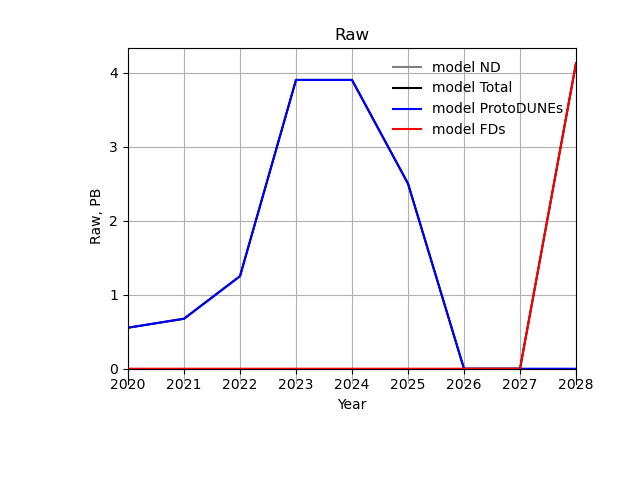
\includegraphics[height=0.4\textwidth]{report/Parameters_2022-11-07-2028-Raw.png}\label{Raw}
\caption{Raw data written per year in PB}
\end{figure}
\begin{figure}[ht]
\centering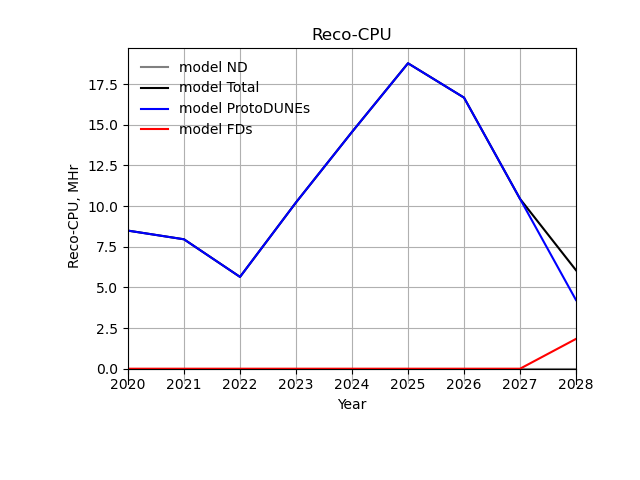
\includegraphics[height=0.4\textwidth]{report/Parameters_2022-11-07-2028-Reco-CPU.png}\label{Reco-CPU}
\caption{CPU needs in core-years for data reconstruction.              Slot weighted wall time takes into account memory use.  Assumes rereconstruction of older data.}
\end{figure}
\begin{figure}[ht]
\centering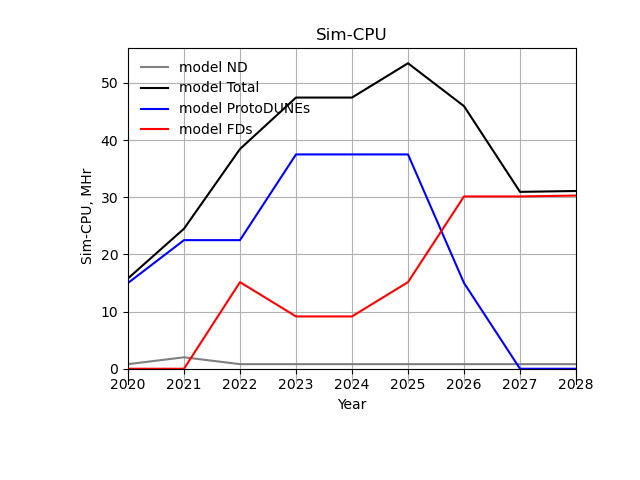
\includegraphics[height=0.4\textwidth]{report/Parameters_2022-11-07-2028-Sim-CPU.png}\label{Sim-CPU}
\caption{CPU needs in core-years for simulation and reconstruction.              Slot weighted wall time takes into account memory use.}
\end{figure}
\begin{figure}[ht]
\centering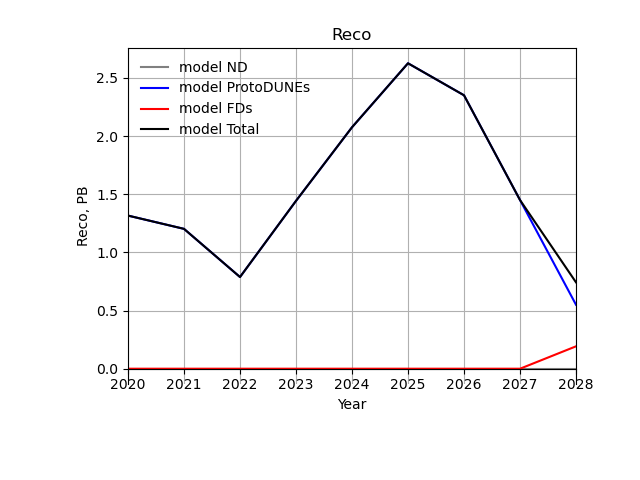
\includegraphics[height=0.4\textwidth]{report/Parameters_2022-11-07-2028-Reco.png}\label{Reco}
\caption{PB of reconstructed files/year}
\end{figure}
\begin{figure}[ht]
\centering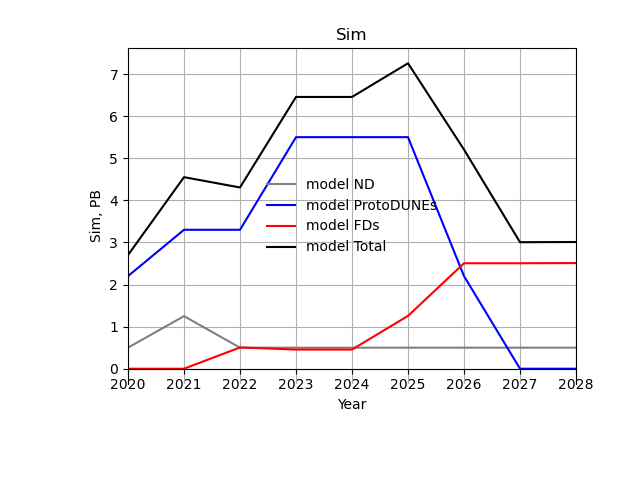
\includegraphics[height=0.4\textwidth]{report/Parameters_2022-11-07-2028-Sim.png}\label{Sim}
\caption{PB of simulated files/year}
\end{figure}
\begin{figure}[ht]
\centering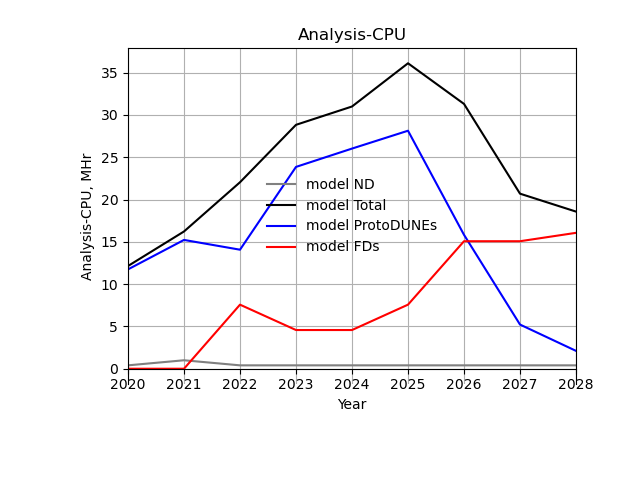
\includegraphics[height=0.4\textwidth]{report/Parameters_2022-11-07-2028-Analysis-CPU.png}\label{Analysis-CPU}
\caption{Analysis CPU needs in core-years.}
\end{figure}
\begin{figure}[ht]
\centering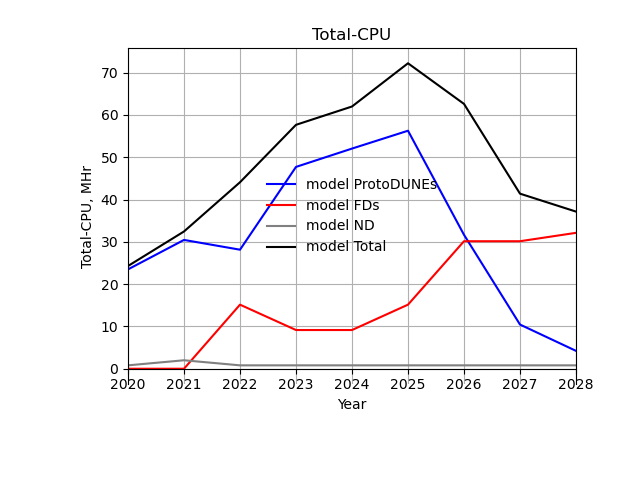
\includegraphics[height=0.4\textwidth]{report/Parameters_2022-11-07-2028-Total-CPU.png}\label{Total-CPU}
\caption{Total CPU needs in core-years. Slot weighted wall time takes into account memory use.}
\end{figure}
\begin{figure}[ht]
\centering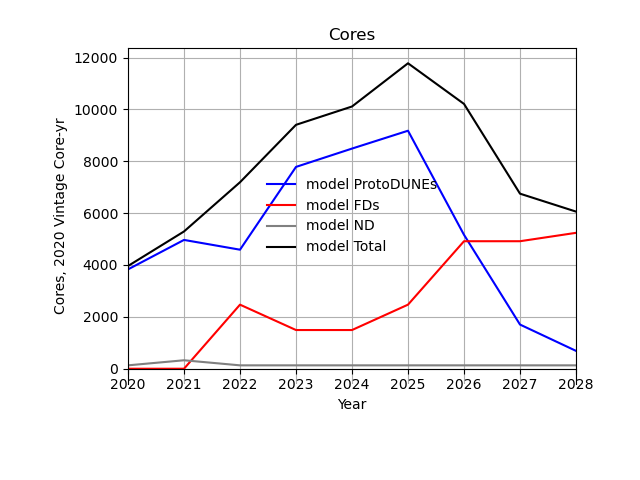
\includegraphics[height=0.4\textwidth]{report/Parameters_2022-11-07-2028-Cores.png}\label{Cores}
\caption{}
\end{figure}
\begin{figure}[ht]
\centering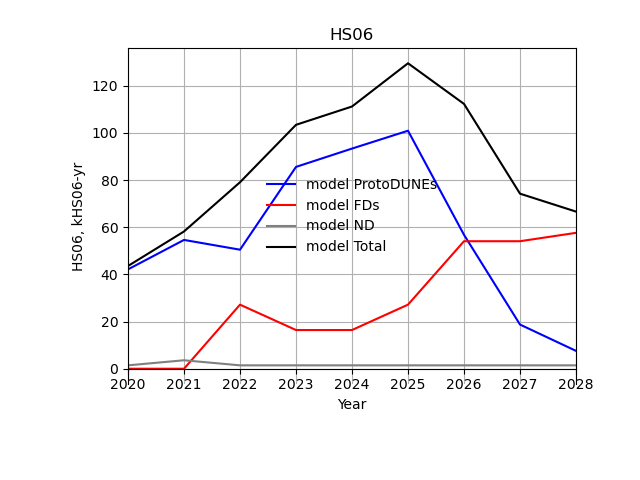
\includegraphics[height=0.4\textwidth]{report/Parameters_2022-11-07-2028-HS06.png}\label{HS06}
\caption{}
\end{figure}
\begin{figure}[ht]
\centering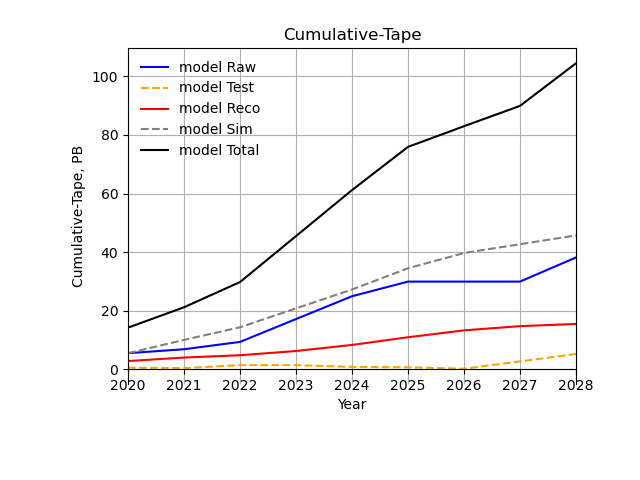
\includegraphics[height=0.4\textwidth]{report/Parameters_2022-11-07-2028-Cumulative-Tape.png}\label{Cumulative-Tape}
\caption{Cumulative Tape needs in PB. Includes data lifetimes}
\end{figure}
\begin{table}[h]
\centering\csvautotabularright{report/Table-Cumulative-Tape.csv}\label{Cumulative-Tape
}
\caption{Cumulative Tape needs in PB. Includes data lifetimes}
\end{table}
\begin{figure}[ht]
\centering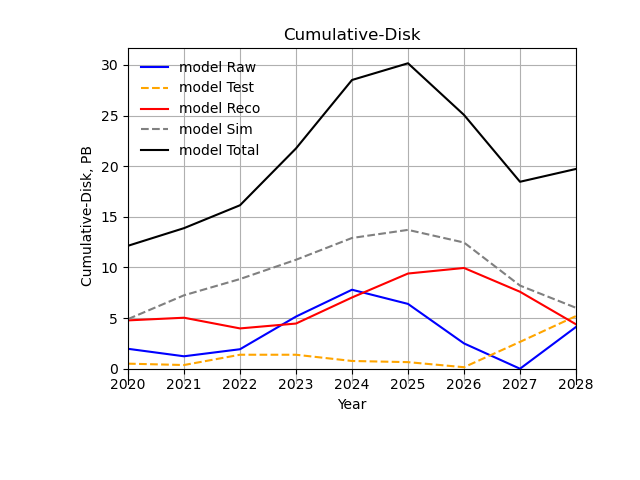
\includegraphics[height=0.4\textwidth]{report/Parameters_2022-11-07-2028-Cumulative-Disk.png}\label{Cumulative-Disk}
\caption{Cumulative Tape needs in PB. Includes data lifetimes}
\end{figure}
\begin{table}[h]
\centering\csvautotabularright{report/Table-Cumulative-Disk.csv}\label{Cumulative-Disk
}
\caption{Cumulative Tape needs in PB. Includes data lifetimes}
\end{table}
{\tt Detectors:} Detectors included in the calculation = {\tt ['SP', 'SP2', 'DP', 'PDVD', 'HD', 'VD', 'ND']} \\
{\tt Cap:} Cap on Raw data/year in PB = {\tt 30} \\
{\tt Base-Memory:} MB of memory per slot assumed as the average = {\tt 2000} \\
{\tt MaxYear:} Plot until year = {\tt 2027} \\
{\tt MinYear:} Plot starting with year = {\tt 2021} \\
{\tt Reprocess:} Number of years of data reprocessed when doing a new pass = {\tt {'SP': 3, 'DP': 2, 'SP2': 4, 'PDVD': 4, 'PDs': 3, 'VD': 100, 'HD': 100, 'FDs': 100, 'ND': 100, 'MARS': 1}} \\
{\tt PatternFraction:} Fraction of time taken in pattern recognition = {\tt {'SP': 0.7, 'SP2': 0.7, 'DP': 0.7, 'PDVD': 0.7, 'PDs': 0.7, 'HD': 0.1, 'VD': 0.1, 'FDs': 0.1, 'ND': 0.9, 'MARS': 0}} \\
{\tt TapeLifetimes:} Number of years kept on tape = {\tt {'Raw-Store': 100, 'Test': 0.5, 'Reco-Data-Store': 15, 'Sim-Store': 15}} \\
{\tt DiskLifetimes:} Number of years kept on disk = {\tt {'Raw-Store': 1, 'Test': 0.5, 'Reco-Data-Store': 2, 'Sim-Store': 2}} \\
{\tt TapeCopies:} Number of copies kept on tape = {\tt {'Raw-Store': 2, 'Test': 1, 'Reco-Data-Store': 1, 'Sim-Store': 1}} \\
{\tt DiskCopies:} Number of copies kept on disk = {\tt {'Raw-Store': 1, 'Test': 1, 'Reco-Data-Store': 2, 'Sim-Store': 1.5}} \\
{\tt PerYear:} Number of reprocessing done per year = {\tt {'Raw-Store': 1, 'Test': 1, 'Reco-Data-Store': 1, 'Sim-Store': 1, 'Events': 1, 'Sim-Events': 1, 'Reco-Data-CPU': 1, 'Sim-CPU': 1, 'Analysis': 1, 'Analysis-CPU': 1}} \\
{\tt Cores:} Description of cores, efficiency and speed relative to 2020 vintage = {\tt {'Efficiency': 0.7, '2020Units': 1}} \\
{\tt kHEPSPEC06PerCPU:} kHEPSPEC06 per core assumed = {\tt 0.011} \\
{\tt SplitsYear:} Year CERN no longer responsible for disk or tape = {\tt 2029} \\
{\tt SplitsEarly:} Division between FNAL/CERN/National for storage until SplitsYear = {\tt {'Tape': {'Raw-Store': {'FNAL': 0.5, 'CERN': 0.5, 'National': 0.0}, 'Sim-Store': {'FNAL': 1.0, 'CERN': 0.0, 'National': 0.0}, 'Reco-Data-Store': {'FNAL': 1.0, 'CERN': 0.0, 'National': 0.0}, 'Test': {'FNAL': 0.5, 'CERN': 0.5, 'National': 0.0}}, 'Disk': {'Raw-Store': {'FNAL': 0.5, 'CERN': 0.5, 'National': 0.0}, 'Sim-Store': {'FNAL': 0.4, 'CERN': 0.1, 'National': 0.5}, 'Reco-Data-Store': {'FNAL': 0.4, 'CERN': 0.1, 'National': 0.5}, 'Test': {'FNAL': 0.5, 'CERN': 0.5, 'National': 0.0}}, 'CPU': {'CPU': {'FNAL': 0.4, 'CERN': 0.1, 'National': 0.5}}}} \\
{\tt SplitsLater:} Division between FNAL/CERN/National for storage after SplitsYear = {\tt {'Tape': {'Raw-Store': {'FNAL': 0.5, 'CERN': 0.0, 'National': 0.5}, 'Sim-Store': {'FNAL': 0.5, 'CERN': 0.0, 'National': 0.5}, 'Reco-Data-Store': {'FNAL': 0.5, 'CERN': 0.0, 'National': 0.5}, 'Test': {'FNAL': 0.5, 'CERN': 0.0, 'National': 0.5}}, 'Disk': {'Raw-Store': {'FNAL': 1.0, 'CERN': 0.0, 'National': 0.0}, 'Sim-Store': {'FNAL': 0.25, 'CERN': 0.0, 'National': 0.75}, 'Reco-Data-Store': {'FNAL': 0.25, 'CERN': 0.0, 'National': 0.75}, 'Test': {'FNAL': 0.5, 'CERN': 0.0, 'National': 0.5}}, 'CPU': {'CPU': {'FNAL': 0.5, 'CERN': 0.0, 'National': 0.5}}}} \\
{\tt filename:} Input configuration file = {\tt MoreSim\_2023-01-31-2040.json} \\

\end{document}
